\documentclass[letterpaper,12pt,fleqn]{article}
\usepackage{matharticle}
\pagestyle{empty}

\begin{document}

\section*{Counting}

\begin{itemize}[left=0in]

\item The archaeological record contains sticks/bones with marks on them, indicating that prehistoric man was
  counting.
  \begin{center}
    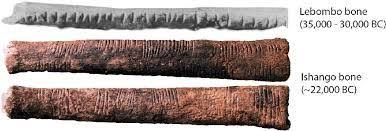
\includegraphics{bones}
  \end{center}

\item When counting, each object in the real world is associated with a mark on the tally stick.
  \begin{center}
    \begin{tikzpicture}
      \node (S1) at (0,4) {
\includegraphics[scale=0.5]{sheep}};
      \node (S2) at (2,4) {
\includegraphics[scale=0.5]{sheep}};
      \node (S3) at (4,4) {
\includegraphics[scale=0.5]{sheep}};
      \node (S4) at (6,4) {
\includegraphics[scale=0.5]{sheep}};
      \draw (0,0) rectangle (8,1);
      \foreach \i in {1,2,3,4}{
        \draw [red] (\i,0.25) -- (\i,0.75);
      }
      \draw [dashed,->] (S1) to (1,0.75);
      \draw [dashed,->] (S2) to (2,0.75);
      \draw [dashed,->] (S3) to (3,0.75);
      \draw [dashed,->] (S4) to (4,0.75);
    \end{tikzpicture}
  \end{center}

\item When more objects are added into the group, extra marks are added to the tally stick.
  \begin{center}
    \begin{tikzpicture}
      \node (S1) at (0,4) {
\includegraphics[scale=0.5]{sheep}};
      \node (S2) at (2,4) {
\includegraphics[scale=0.5]{sheep}};
      \node (S3) at (4,4) {
\includegraphics[scale=0.5]{sheep}};
      \node (S4) at (6,4) {
\includegraphics[scale=0.5]{sheep}};
      \node (S5) at (8,4) {
\includegraphics[scale=0.5]{sheep}};
      \node (S6) at (10,4) {
\includegraphics[scale=0.5]{sheep}};
      \draw (0,0) rectangle (8,1);
      \foreach \i in {1,2,3,4}{
        \draw [red] (\i,0.25) -- (\i,0.75);
      }
      \foreach \i in {5,6}{
        \draw [green] (\i,0.25) -- (\i,0.75);
      }
      \draw [dashed,->] (S1) to (1,0.75);
      \draw [dashed,->] (S2) to (2,0.75);
      \draw [dashed,->] (S3) to (3,0.75);
      \draw [dashed,->] (S4) to (4,0.75);
      \draw [dashed,->] (S5) to (5,0.75);
      \draw [dashed,->] (S6) to (6,0.75);
    \end{tikzpicture}
  \end{center}

\item Thus, the tally stick mirrors reality: operations on the tally stick can be used to describe past and current
  states and make predictions about future states.

\item We use the real number line in the same way, but instead of counting discrete objects we typically measure
  (seemingly) continuous phenomena (e.g., the height of a falling object, population growth).

\end{itemize}

\end{document}
